\glsresetall{} 
\appendix

\chapter{Algorithms}

Through the development of the \gls{pops}, a number of algorithms have been
developed to perform various functions. These algorithms are not necessarily
ground breaking but their implementations are novel and worth discussing in
some form. To avoid detracting from the main body of the thesis they have been
placed here, in the appendices.


\section{Algorithm 1: Multiple Access Intersection} 

For some search scenarios, we may need to determine for what times do all
satellites have access to a target such as an \gls{aoi} or a ground station.
That is, if we have more than one satellite and each satellite has a list of
access times to a target, we must generate a new list of access times where
each access corresponds to a period where all satellites have access. An
example scenario is illustrated in Figure \ref{fig:access_intersect}.


\begin{figure}[h]
    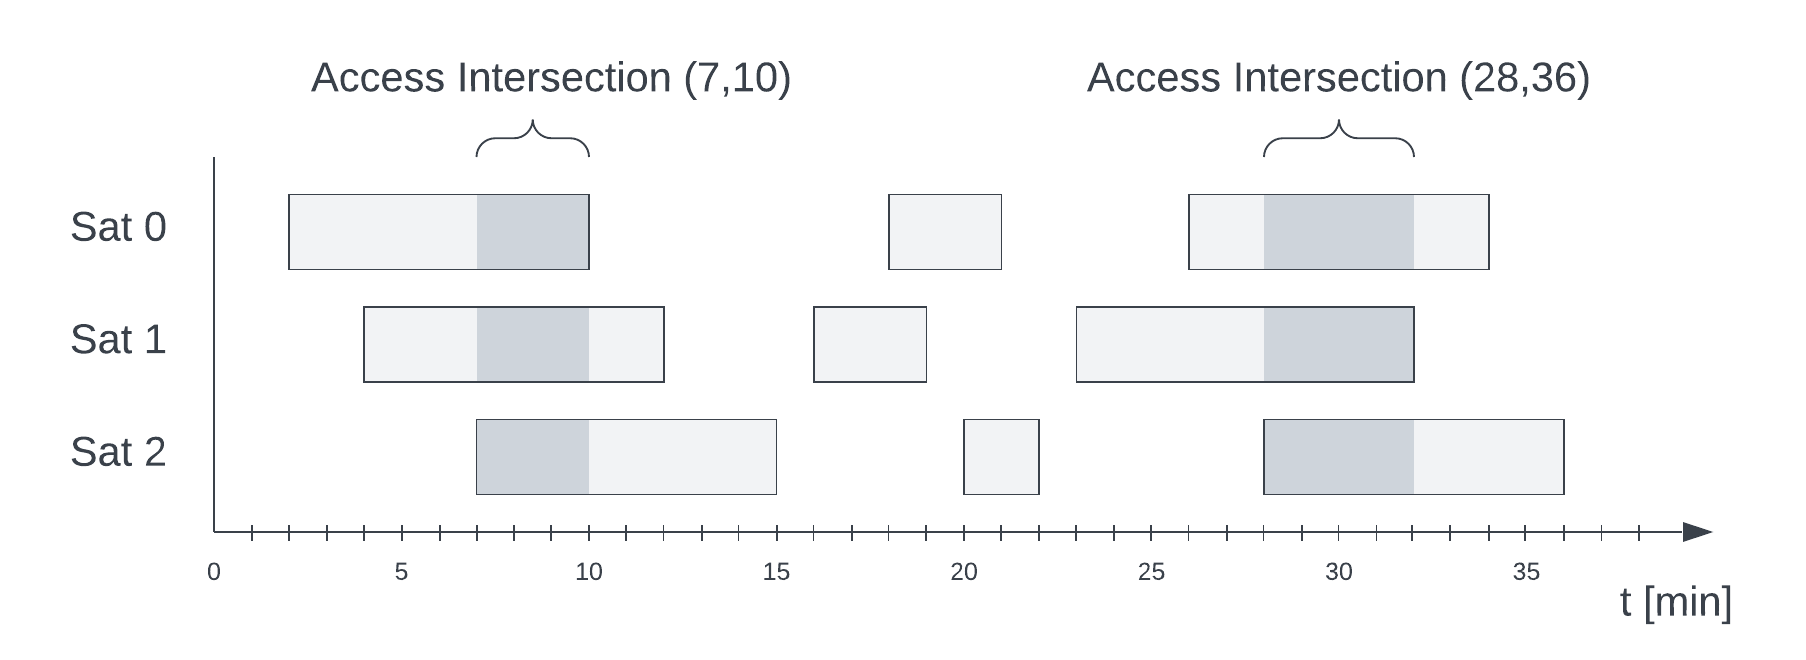
\includegraphics[width=\textwidth]{Access Intersection Example.png} 
    \caption{Illustration of a Potential Access Intersection Scenario}
\label{fig:access_intersect}
\end{figure}

In this scenario, there are three satellites: Sat 0, Sat 1, and Sat 2. Each has
multiple access periods represented with grey boxes. Though time is continuous,
it has been discretized into integer timesteps for simplicity. Minutes have
been selected as the units for time but this is arbitrary. From these lists of
access periods, this algorithm must determine all of the points in time where
all satellites have an access period. For the example scenario, the outputted
results should be $[7,10]$ and $[28,36]$. Note that between $t = 16$ and $t=22$
there are access overlaps but since there are only overlaps between two
satellites, they should not be returned as intersection periods.

For a satellite, access times are stored as a list of timestamps. Every even
and odd indexed timestamp specifies when the satellite `enters' and `leaves' an
access respectively. Access lists $\ses{a}{n}$ can be described generally for satellite $n$ as,

\begin{equation} 
    \ses{a}{n} = \left[ a_{n,0}, b_{n,0}, a_{n,1}, b_{n,1}, \ldots a_{n,m}, b_{n,m} \right]
\end{equation}


where $a$ is the access enter timestamp, $b$ is the access leave timestamp, and
$m$ is the number of accesses. We also make the assumption that no accesses
overlap for a given satellite and target; that is,

\[
    a_{n,0} < b_{n,0} < a_{n,1} < b_{n,1} < \ldots < a_{n,m} < b_{n,m}
\]

One simple brute force solution to this problem would be to iterate over every
time step, $t$, and check if there exists an access region, $[a_n,b_n]$, for all
satetellites, $n$, such that $t$ is between $a$ and $b$. Put succinctly,


This solution is, of course, very wasteful as it scales with the number of
timesteps that are being considered, $\Theta(t)$. The number of timesteps maybe
on the order of 100s to 10,000s of timesteps. A simplification can be made
since we do not need to actually consider every timestep. Rather, we can
instead iterate over the access boundaries since they describe continuous
periods of time. By focusing on just the access boundaries, we may develop an
algorithm which scales with the number of accesses, $\Theta(m)$, which is much
smaller than the totalnumber of timesteps.

For all satellite access lists we are considering, let us combine them into two
$1\times nm$ arrays. The first `timestamp' array, $\se{b}$, contains a sorted
list of all of the boundary timestamps in ascending order. The second `index'
array, $\se{s}$, contains a list of satellite indeces in the same order as the
timestamp array. For example,

\begin{equation*}
    \begin{aligned} 
	\ses{a}{0} &= \left[ 2, 10, 18, 21  \right] \\
	\ses{a}{1} &= \left[ 4, 12, 16, 19  \right] \\
	\ses{a}{2} &= \left[ 7, 15, 20, 22  \right] \\
    \end{aligned}
    \quad \Rightarrow \quad
    \left \{ 
	\begin{aligned}
	    \se{b} &= [ 2 , 4 , 7 , 10 , 12 , 15 , 16 , 18 , 19 , 20 , 21 , 22  ] \\
	    \se{s} &= [ 0 , 1 , 2 , 0 , 1 , 2 , 1 , 0 , 1 , 2 , 0 , 2  ]
	\end{aligned}
    \right.
\end{equation*}

Note these are some of the values from Figure \ref{fig:access_intersect}.
Again, in the actual implementation of the algorithm we use actual timestamps,
but here we are using integers for demonstration purposes. The timestamp array
stores the timestamp of the access boundary for later reference and also gives
us the order of the satellite index array. Now with the index array we can do
something interesting. Remember that access boundaries are listed in order of
[enter, leave, enter, leave, etc.]. Looking at the first four elements in the
index array, $[0, 1, 2, 0]$, satellite 0 enters an access at the first element
and leaves the access at the fourth element. So for the second and third
element, satellite 0 still has access because it has not left yet. In essence,
the index array encodes in what order satellites enter and leave accesses. 

Now let us expand on the index array so we can perform logical operations to
find intersections. For this make use of logic arrays.  These are arrays which
contain only boolean values, True or False. With these arrays, we can also
perform logical operations on any axis. For example, if we have a 2 dimensional
logic array, we can produce a 1 dimensional array, that is the result of
AND'ing all of the elements in each column. These allow us to perform logical
operations very quickly for many elements. From the index array let us
construct an $n\times nm$ boolean array that describes our scenario, $\se{A}$.
The rows of matrix, $\se{A}$, corrspond to the indeces of each satellite.  For
example row 0 is satellite 0, row $m$ is satellite $m$, etc. The columns
correspond to elements in the index array, $\se{s}$.

Let us initialize $\se{A}$ to be all False represented as 0s. Then, starting at
the first column of $\se{A}$, let us NOT the element in the $\se{s}(0)$ row.
Then, for then next column, let us copy all of the values from the previous
column and again NOT the $\se{s}(1)$ element. This is then repeated for all
columns in $\se{A}$. There is one small catch, if we are transitioning a 1 to a
0 or a True to a False, this should be done on the following iteration. This
essentially means that we are treating accesses in in access boundaries as
inclusive. Even if the satellite is leaving an access, we say that it has
access until the timestep imediately after the boundary. As an example, let us
construct $\se{A}$ from $\se{s}$ for all of Figure \ref{fig:access_intersect},

\begin{equation*} 
    \se{s} = 
    \left[
    \begin{array}{cccccccccccccccccc}
	0 & 1 & 2 & 0 & 1 & 2 & 1 & 0 & 1 & 2 & 0 & 2 & 1 & 0 & 2 & 1 & 0 & 2 \\
    \end{array}
    \right]
\end{equation*}
yields,
\begin{equation*} 
    \se{A} = 
    \left[
	\begin{array}{cc;{2pt/2pt}cc;{2pt/2pt}cccccccccc;{2pt/2pt}cc;{2pt/2pt}cc}
	1 & 1 & 1 & 1 & 0 & 0 & 0 & 1 & 1 & 1 & 1 & 0 & 0 & 1 & 1 & 1 & 1 & 0 \\
	0 & 1 & 1 & 1 & 1 & 0 & 1 & 1 & 1 & 0 & 0 & 0 & 1 & 1 & 1 & 1 & 0 & 0 \\
	0 & 0 & 1 & 1 & 1 & 1 & 0 & 0 & 0 & 1 & 1 & 1 & 0 & 0 & 1 & 1 & 1 & 1 \\
    \end{array}
    \right]
\end{equation*}
Then, if we AND all of the rows in $\se{A}$ we get,
\begin{equation*} 
    \se{A}' = 
    \left[
    \begin{array}{cccccccccccccccccc}
	0 & 0 & 1 & 1 & 0 & 0 & 0 & 0 & 0 & 0 & 0 & 0 & 0 & 0 & 1 & 1 & 0 & 0 \\
    \end{array}
    \right]
\end{equation*}
Now it is clear to see that this matrix gives us the indeces where there is an
intersection between all satellites. If we take all values of $\se{b}$ where
$\se{A}'$ is True, we are left with,
\begin{equation*} 
    \se{b}' = 
    \left[
    \begin{array}{cccccccccccccccccc}
	7 & 10 & 28 & 32
    \end{array}
    \right]
\end{equation*}
Which is our expected result. This was just a walkthrough but the explicit
alogrithm definition is as follows,

\begin{algorithm}[h] 
    \caption{Access Intersection} 
    \label{alg:access-intersection}
    \begin{algorithmic}[1]
	%\Require{\se{z}is a $1\times N$ array } 
	\Function{AccessIntersection}{$\ses{a}{0}$,$\ses{a}{1}$, ... , $\ses{a}{n}$} 

	    \Let{$\se{s}$, $\se{b}$}{\Call{Combine}{$\ses{a}{0}$,$\ses{a}{1}$, ... , $\ses{a}{n}$}}  

	    \Let{$l$}{\Call{Length}{$\se{s}$}}

	    \Let{$\se{A}$}{\Call{Zeros}{$n$,$l$}}

	    %\Let{$\se{A}[\se{s}[0],0]$}{1}  \Comment{Set up the first column}
	    \Let{$temp$}{$\se{A}[:,0]$} \Comment{Temporary array to store column of $\se{A}$}

	    \Let{$i$}{0} \Comment{Boundary iterator}

	    \While{$i \neq m$}
		\Let{$s$}{$\se{s}[i]$} \Comment{Satellite index}
		
		\If{!$temp$($s$)}
		    \Let{$temp$($s$)}{!$temp$($s$)}
		    \Comment{Flip element then copy values over}
		    \Let{$\se{A}[:,s]$}{\Call{OR}{$\se{A}[:,s]$, $temp$}} 
		\Else
		    \Let{$\se{A}[:,s]$}{\Call{OR}{$\se{A}[:,s]$, $temp$}} 
		    \Comment{Copy values over then flip element}
		    \Let{$temp$($s$)}{!$temp$($s$)}
		\EndIf


		\Let{$i$}{$i+1$}
	    \EndWhile 

	    \Let{$\se{A}'$}{\Call{ColumnsAND}{$\se{A}$}}

	    \Let{$\se{b}'$}{$\se{b}[\se{A}']$}

	\State \Return $\se{b}'$
	\EndFunction
    \end{algorithmic}

\end{algorithm}

 




